\documentclass[tikz, margin=1mm]{standalone}

\usetikzlibrary{matrix}
\usetikzlibrary{positioning}
\usetikzlibrary{patterns}
\usetikzlibrary{decorations.markings}
\usetikzlibrary{arrows}
\usetikzlibrary{arrows.meta}
\usetikzlibrary{backgrounds}
\usetikzlibrary{math}

\definecolor{textColor}{RGB}{248, 248, 255}
\definecolor{bgColor}{RGB}{29, 32, 38}

\begin{document}
    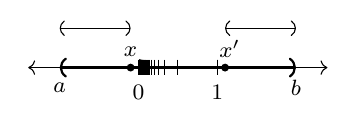
\begin{tikzpicture}
        \draw[<->] (-1.4,0) -- (2.4,0);
        \draw[(-)] (-1,0.5) -- (-0.1,0.5);
        \fill (-0.1,0) circle (0.05);
        \draw (-0.1,0.2) circle (0) node{\footnotesize{$x$}};
        \draw[(-)] (1.1,0.5) -- (2,0.5);
        \fill (1.1,0) circle (0.05);
        \draw (1.16,0.24) circle (0) node{\footnotesize{$x'$}};
        \draw[(-), thick] (-1,0) -- (2,0);
        \draw (-1,-0.26) circle (0) node{\footnotesize{$a$}};
        \draw (2,-0.26) circle (0) node{\footnotesize{$b$}};
        \draw (0,0.1) -- (0,-0.1) node[anchor=north]{\footnotesize{$0$}};
        \draw (1,0.1) -- (1,-0.1) node[anchor=north]{\footnotesize{$1$}};
        \foreach \i in {1,...,100}
        {
            \tikzmath
            {
                \x = 1 / \i;
            }
            \draw (\x,0.1) -- (\x, -0.1);
        }
    \end{tikzpicture}
\end{document}
